% 固定来源PDF第2页第11题的四个定性选项图。
% 各面板只示意曲线方向及直线截距所在区间，不声明未给出的精确绘图比例。
% 只有C使用同一个 0<a<1 同时满足 y=x+a 与 y=log_a(x)。
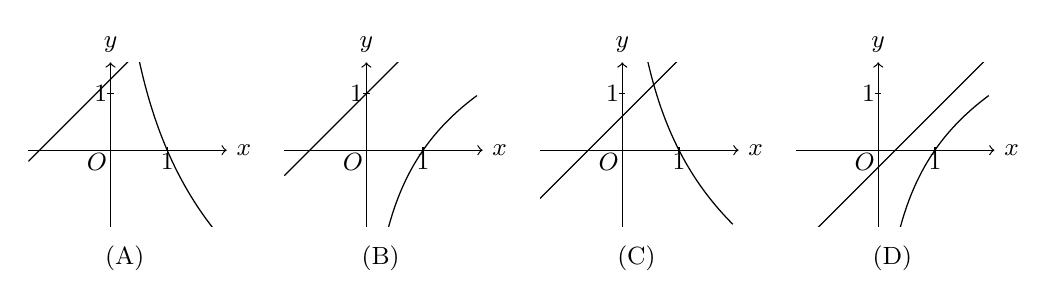
\begin{tikzpicture}[line width=.45pt,x=.72cm,y=.72cm,font=\small]
  \foreach \panel/\shift/\linea/\loga in {A/0/1.25/.65,B/3.25/1/2,C/6.5/.6/.6,D/9.75/-.3/2}{
    \begin{scope}[xshift=\shift cm]
      \begin{scope}
        \clip (-1.45,-1.35) rectangle (2.05,1.55);
        \draw[domain=.34:1.95,samples=70,smooth] plot (\x,{ln(\x)/ln(\loga)});
        \draw[domain=-1.45:2.05,samples=2] plot (\x,{\x+\linea});
      \end{scope}
      \draw[->] (-1.45,0)--(2.05,0) node[right] {$x$};
      \draw[->] (0,-1.35)--(0,1.55) node[above] {$y$};
      \draw (-.055,1)--(.055,1);
      \node[left,inner sep=1pt] at (0,1) {$1$};
      \draw (1,-.055)--(1,.055);
      \node[below,inner sep=1pt] at (1,0) {$1$};
      \node[below left,inner sep=1pt] at (0,0) {$O$};
      \node at (.25,-1.9) {(\panel)};
    \end{scope}
  }
\end{tikzpicture}
